%!TEX root = ../Thesis.tex
\chapter{Results and analysis}
\label{chap:result}
This chapter presents the results from benchmarking the real-time GPU resource monitoring and alerting system in experimental and production setups. The evaluation includes a comprehensive analysis of the system's performance, scalability, and impact on energy efficiency and resource utilization for production within High-Performance Computing (HPC) clusters.

\section{Benchmark}
\subsection{Experimental setup}
\label{subsection:experiment}
The experimental setup involves deploying the proposed GPU monitoring system in a controlled environment, that emulates the characteristics of a typical HPC cluster. The monitoring infrastructure continuously collects and analyzes the simulated GPU metrics, and an alert service is configured to notify any sub-optimal GPU utilization.

To integrate all the components for testing, we deployed Slurm in a containerized environment with an isolated network to simulate the actual HPC job context. Everything, including the software versions, replicates what we have in production. We use Podman as the container runtime and Rocky Linux 8 as the base container image to keep up with the operating system we use in Puhti and Mahti (RHEL 8).

We have two compute nodes in our test environment. All the containers are listed as follows:
 
\begin{itemize}
    \item \textbf{mysql}: Database for Slurm to store job data.
    \item \textbf{slurmctld}: Central controller daemon of Slurm monitors all other Slurm daemons and resources, accepts jobs, and allocates resources.
    \item \textbf{slurmdbd}: Interface to the MySQL database for Slurm can be used to archive accounting records.
    \item \textbf{cpn01}: Compute node 1 for executing actual jobs received by Slurm.
    \item \textbf{cpn02}: Compute node 2 for executing actual jobs received by Slurm.
    \item \textbf{frontend}: Similar to the login node in HPC for submitting jobs.
    \item \textbf{timescaledb}: TimescaleDB instance for storing the monitoring data.
    \item \textbf{timescaleingest}: Timescale Ingest instance for ingesting the monitoring data into TimescaleDB.
    \item \textbf{timescalereader}: Timescale Reader instance for fetching the monitoring data and serving as the API for displaying to end users.
    \item \textbf{timescalealert}: Timescale Alert instance for checking alerts and displaying related information.
    \item \textbf{ondemand}: Open OnDemand serves as a web-based UI to computer clusters in HPC, in addition to SSH access, to help new users who are not familiar with Linux get started quickly. It offers an intuitive entry point for straightforward tasks and shell access for more intricate operations.
    \item \textbf{ldap}: Lightweight Directory Access Protocol (LDAP), for access control in Open OnDemand.
\end{itemize}

To make testing easier with an arbitrary number of GPUs in a container without needing them, we created a fake Nvidia library that implements the Nvidia-ML interface for generating random data.

We also have separate testing setups for each component, either by randomly generated data or by replaying the data we collected in production from the database dump.

\begin{itemize}
    \item For the random data benchmark, we spawn maximum 23824 (2978*8) Go routines that write to the database simultaneously, which is, i.e., the maximum GPU number we have in LUMI, to simulate the heaviest situation we can have in the pre-exascale supercomputer.
    \item For real data replaying, we read all the records from the database dump ordered by time stamp, and send it to timescale ingest with accelerated speed to reproduce the production situation.
\end{itemize}

\subsection{Performance}
\label{subsec:performance}
The benchmarking process focused on evaluating the system's responsiveness in detecting anomalies and the overall impact on system performance during monitoring, to assess the system's adaptability and robustness in different usage patterns.

We use the local environment to run the container setup mentioned in Subsection \ref{subsection:experiment} on the 12th Gen Intel Core i7-12700H CPU with SSD and 16 GB of RAM by writing random GPU metrics data to the database continuously in an infinite loop, without any interval for writing and dumping data. We run each solution for 10 minutes and take the average of the last 2-minute delay. The benchmark result is shown in Figure \ref{fig_benchmark}:

% import matplotlib.pyplot as plt

% # Data
% methods = ["Polling CAGG", "Polling Direct Query", "Trigger CAGG", "Trigger in Memory"]
% colors = ["#36A2EB", "#FF6384", "#FF9F40", "#9966FF"]
% gpu_write_delay = [
%     [0.321007643, 0.660196607, 1.279614867, 2.433749516, 5.131623884, 11.624568741],
%     [0.31859915, 0.625456453, 1.191235464, 2.350517039, 4.958478354, 9.977873813],
%     [0.765987412, 1.609155407, 2.73052539, 5.176909349, 10.908855175, 20.96940738],
%     [0.65528452, 1.285481557, 2.53125466, 5.007170087, 9.824896244, 19.604722893]
% ]
% read_iteration = [
%     [1.201504459, 2.102009134, 3.58900885, 7.282948943, 13.567867101, 18.581255946],
%     [2.245655323, 3.443534234, 6.191009134, 12.676023435, 26.139007435, 55.204802484],
%     [13.184558, 30.957367, 56.111442, 101.592729, 212.071778, 433.089509],
%     [12.250112, 30.117734, 52.671703, 91.90153, 188.53631, 388.158221]
% ]
% index = range(len(gpu_write_delay[0]))

% # Plot for GPU Write Delay
% fig, axes = plt.subplots(3, 1, figsize=(8, 12))

% for i, method in enumerate(methods):
%     axes[0].bar([x + i * 0.2 for x in index], gpu_write_delay[i], 0.2, label=method, color=colors[i])

% axes[0].set_xlabel('Node Count * GPU')
% axes[0].set_ylabel('Time (s)')
% axes[0].set_title('Delay in Database Writing Transaction Commit')
% axes[0].set_xticks([x + 0.2 * 3 / 2 for x in index])
% axes[0].set_xticklabels(['93*8', '186*8', '372*8', '744*8', '1489*8', '2978*8'])
% axes[0].legend()

% # Plot for Read Iteration
% for i in range(2):
%     method = methods[i]
%     axes[1].bar([x + i * 0.2 for x in index], read_iteration[i], 0.2, label=method, color=colors[i])

% axes[1].set_xlabel('Node Count * GPU')
% axes[1].set_ylabel('Time (s)')
% axes[1].set_title('Time Needed in Completing a Read Loop Iteration')
% axes[1].set_xticks([x + 0.2 * 3 / 2 for x in index])
% axes[1].set_xticklabels(['93*8', '186*8', '372*8', '744*8', '1489*8', '2978*8'])
% axes[1].legend()

% # Plot for Read Iteration
% for i in range(2, 4):
%     method = methods[i]
%     axes[2].bar([x + i * 0.2 for x in index], read_iteration[i], 0.2, label=method, color=colors[i])

% axes[2].set_xlabel('Node Count * GPU')
% axes[2].set_ylabel('Time (ms)')
% axes[2].set_title('Delay in Completing a Memory Status Dump')
% axes[2].set_xticks([x + 0.2 * 3 / 2 for x in index])
% axes[2].set_xticklabels(['93*8', '186*8', '372*8', '744*8', '1489*8', '2978*8'])
% axes[2].legend()

% plt.tight_layout()
% plt.savefig("benchmark-data.pdf")

\begin{figure}[H]
    \centering
    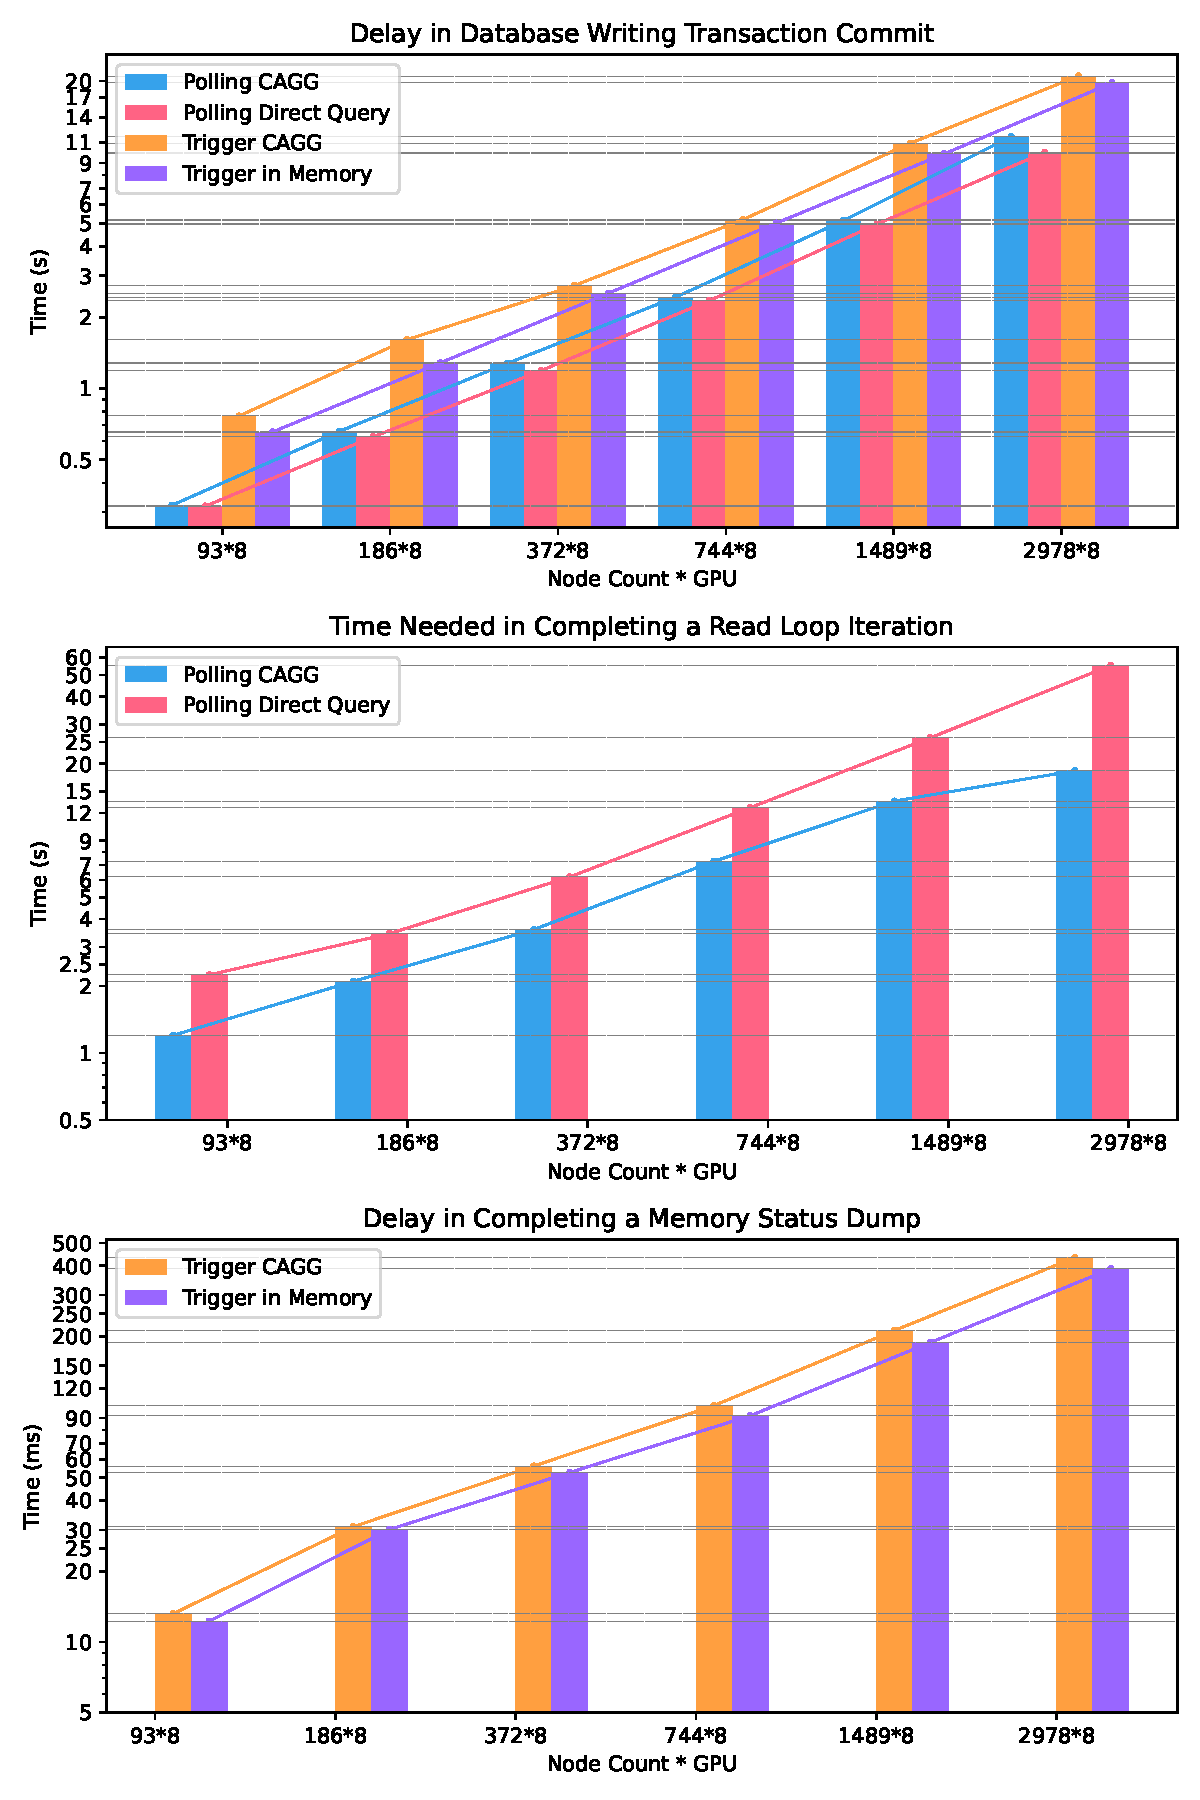
\includegraphics[width=1\textwidth]{figures/benchmark-data.pdf}
    \caption{Timescale Alert benchmark result}
    \label{fig_benchmark}
\end{figure}

From Figure \ref{fig_benchmark}, we can learn that:

\begin{itemize}
    \item Generally, all the delays scale linearly with the number of GPUs.
    \item Triggers generally double the delay in database transaction commit time for writing, which the overhead of NOTIFY should be the cause.
    \item Continuous aggregates (CAgg) cause a slight increase in writing delay and the memory status dump delay for the triggers solution, which is likely to be caused by the overhead of CAgg background jobs. However, CAgg accelerates the query speed dramatically compared to traditional SQL queries aggregate, as we can see a significant time reduction in completing a read loop among all the jobs available.
    \item Polling is very inefficient for accessing data in real-time, since it creates a delay that is almost 100x more than the triggers solution.
\end{itemize}

Hence, the results confirmed our empirical analysis in Section \ref{sec:alertservice} and led to our final design after comparison: \textbf{triggers without continuous aggregates}. The reason is that triggers have the best real-time access, while only doubling the delay in writing compared to polling, which is acceptable, and the in-memory solution has a better performance in both read and write delay. Most importantly, the in-memory solution allows us to access raw data for more complicated statistics calculations and use machine learning models. We used the Golang data race detector to ensure the correctness during benchmarking and testing. We also checked the memory usage during the benchmark: The maximum Resident Set Size (RSS) is around 84.6 MB, which is also acceptable.

%CPU %MEM    VSZ   RSS 21.0  0.5 3184092 84612

\section{Production}

The production evaluation involved deploying the real-time GPU monitoring system in a live HPC environment, including Puhti and Mahti. This evaluation allows us to test the practicability of alerting for real-world workloads from diverse scientific domains, including molecular dynamics simulations, computational chemistry, and machine learning. Unfortunately, due to the time limit for the thesis writing process, we cannot finish deploying the alert services in production for the pre-exascale HPC system, LUMI. Still, we have verified this possibility in Section \ref{subsection:experiment} through a benchmark.

% We intended to deploy this whole infrastructure on LUMI as well. Unfortunately, we were unable to do so during the thesis writing period due to the shortage of administrators on the LUMI side.

The production evaluation focused on the practical implications of integrating the alerting and monitoring system into the daily operations of HPC clusters. Key performance indicators were measured, such as the system's ability to facilitate timely alerts. Additionally, the impact on user experience was evaluated considering the introduction of real-time alerts to administrators.

\subsection{Setup}

As is presented in Figure \ref{fig_monitoring_production_development}, we have two copies of the monitoring infrastructure separately for Puhti and Mahti deployed as microservices inside containers:

\begin{figure}[H]
    \centering
    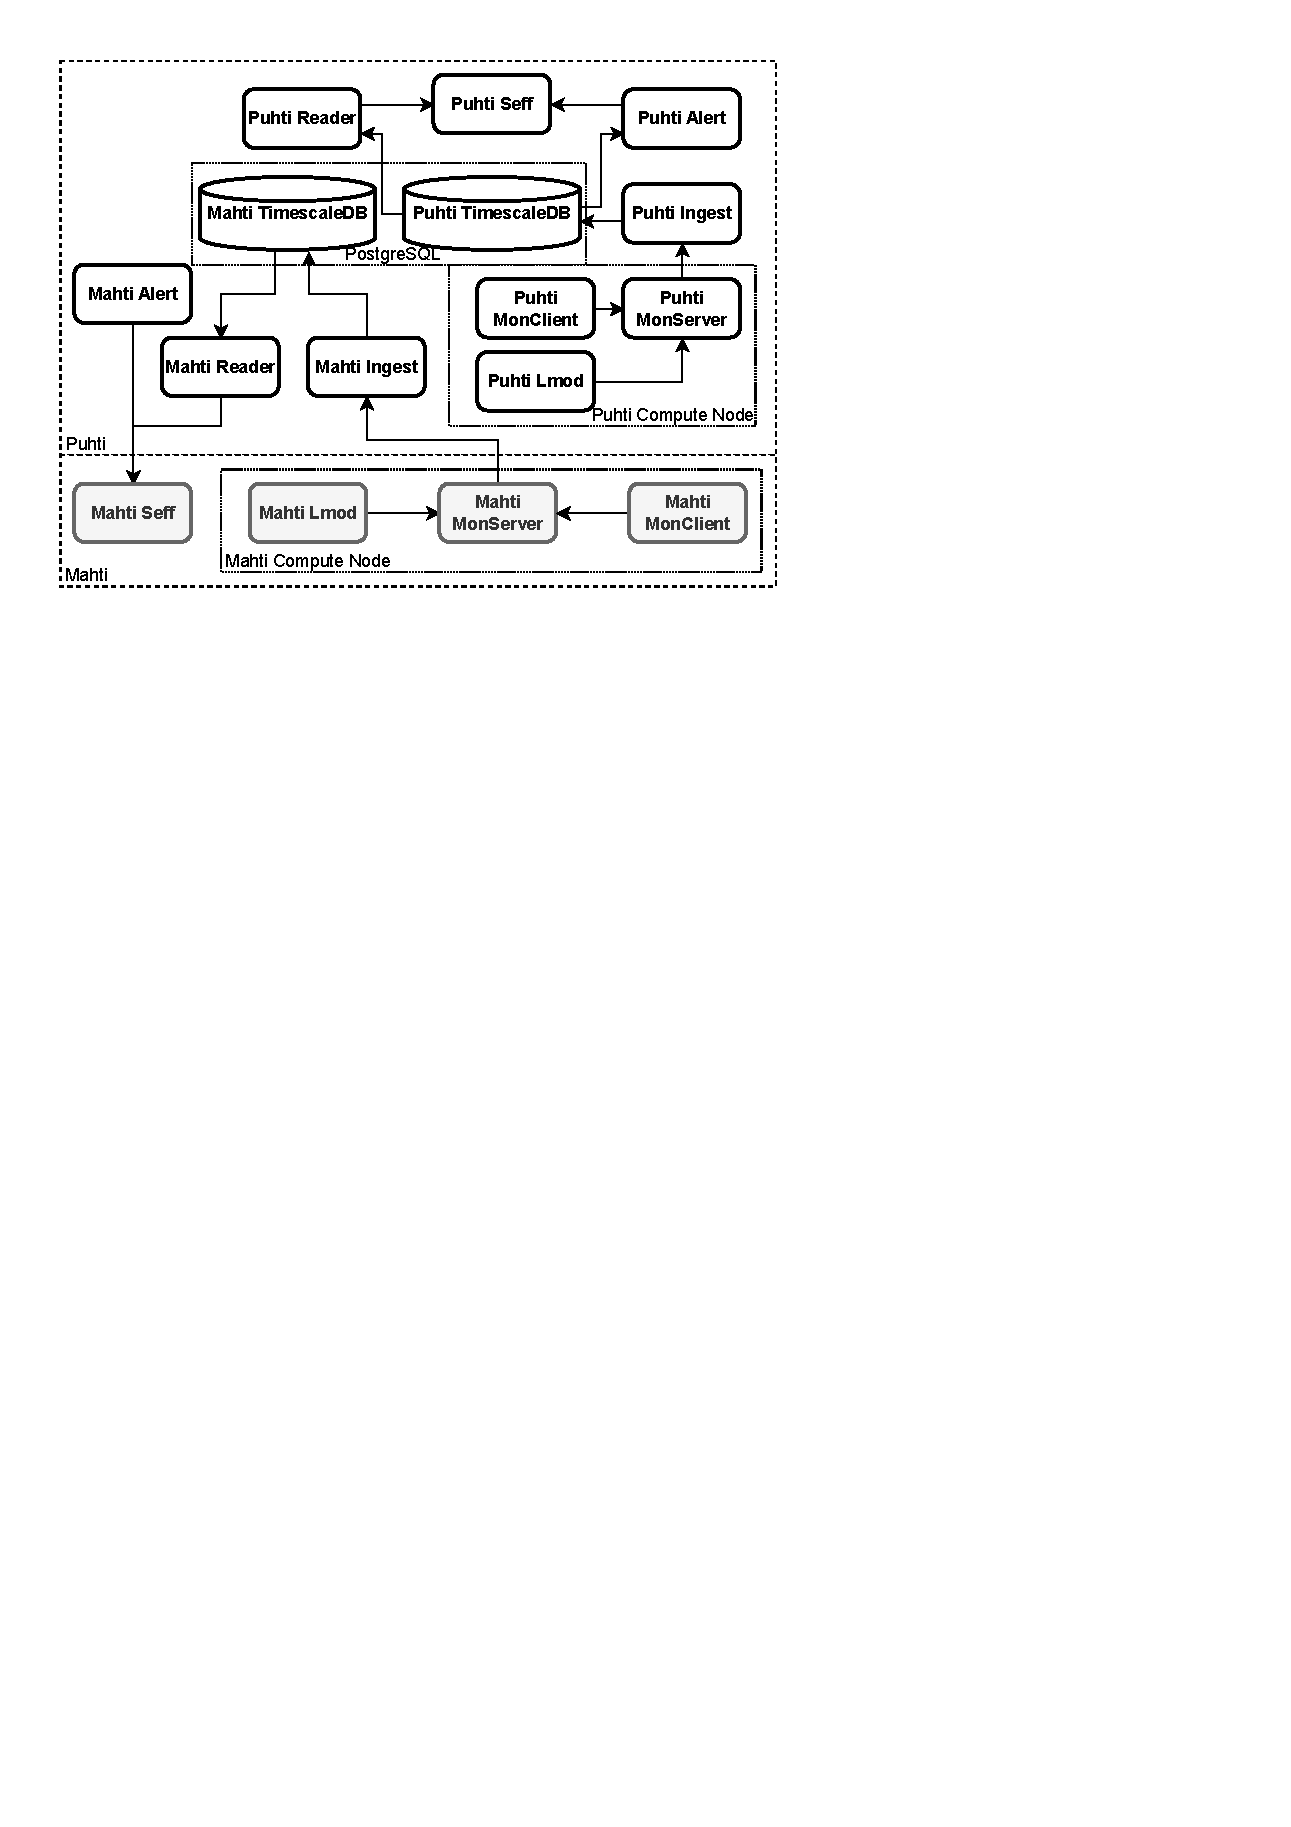
\includegraphics[width=1\textwidth]{figures/production-deployment.pdf}
    \caption{GPU monitoring infrastructure production setup for Puhti and Mahti}
    \label{fig_monitoring_production_development}
\end{figure}

\begin{itemize}
    \item \textbf{Monitoring Daemon} is written in C++ and deployed on each compute node for both Puhti and Mahti. The \textbf{Monitoring Server} is deployed as a systemd service. In contrast, the \textbf{Monitoring Client} is deployed as a CLI utility to be called by the Slurm prolog and epilog scripts.
    \item \textbf{Lmod} is the environment module system in Lua. It is deployed on each compute node as well.
    \item \textbf{Timescale Reader}, \textbf{Timescale Ingest}, and \textbf{Timescale Alert} are all written in Go and deployed as systemd services. Both copies for Mahti and Puhti are deployed on the Puhti MonDB Utility node.
    \item \textbf{TimescaleDB} is deployed as a plugin on the PostgreSQL node. We use different database names to isolate the monitoring data between Puhti and Mahti.
    \item \textbf{Seff} script is the CLI utility written in Perl. It is installed as an RPM package by admins in all the nodes and can be called by the user.
    \item Other \textbf{visualization} services, such as the job history and alert status dashboard, are deployed as Flask Apps for Open OnDemand.
\end{itemize}

We set the alert sliding window size at 30 minutes. Initially, we collected the monitoring data at 1-minute intervals, then increased that to 20 seconds, and the whole monitoring and alert system was still stable enough. We set the compression policy to compress the data after one day and do the retention every half-year. We also put an index on the hostname, job ID, and GPU ID to accelerate the querying speed.

\subsection{Case studies}
Here are some real-world scenarios in which we use our monitoring infrastructure and Timescale Alert to help users solve issues when they submit jobs in HPC. These case studies illustrate how the system proposed in this thesis enables the support team to proactively identify, diagnose, and resolve issues, ensuring efficient utilization of HPC, reducing user queuing time, and improving user satisfaction.

\subsubsection{Configuration Error}
From the GPU alert status dashboard, the user support team was alerted by a job that reserved two full nodes, each with 4 A100 GPUs. It has nearly 100\% usage almost all the time for 1 GPU but zero usage for the remaining 7, as illustrated in Figure \ref{fig_job_config_error}. By checking the GPU alert history dashboard, the support team found that the alert began long ago. The disk I/O currently used by that job is low, so it shouldn't be the case that the job is still loading data. The situation leads them to suspect a configuration error or code bug. By examining the module load information stored in the job metadata, they discovered that Pytorch was loaded into the job context, a mature machine-learning library that shouldn't have such a situation if everything is configured right. The user support team then contacted the user to investigate possible configuration errors. It was eventually discovered that \texttt{CUDA\_VISIBLE\_DEVICES} was mistakenly set to \texttt{0} (utilizing one GPU only), and they didn't use \texttt{srun} to distribute the job steps to all nodes properly with \texttt{torchrun}. The job was terminated to fix this, and a new job with the correct configuration was subsequently submitted.

\begin{figure}[H]
    \centering
    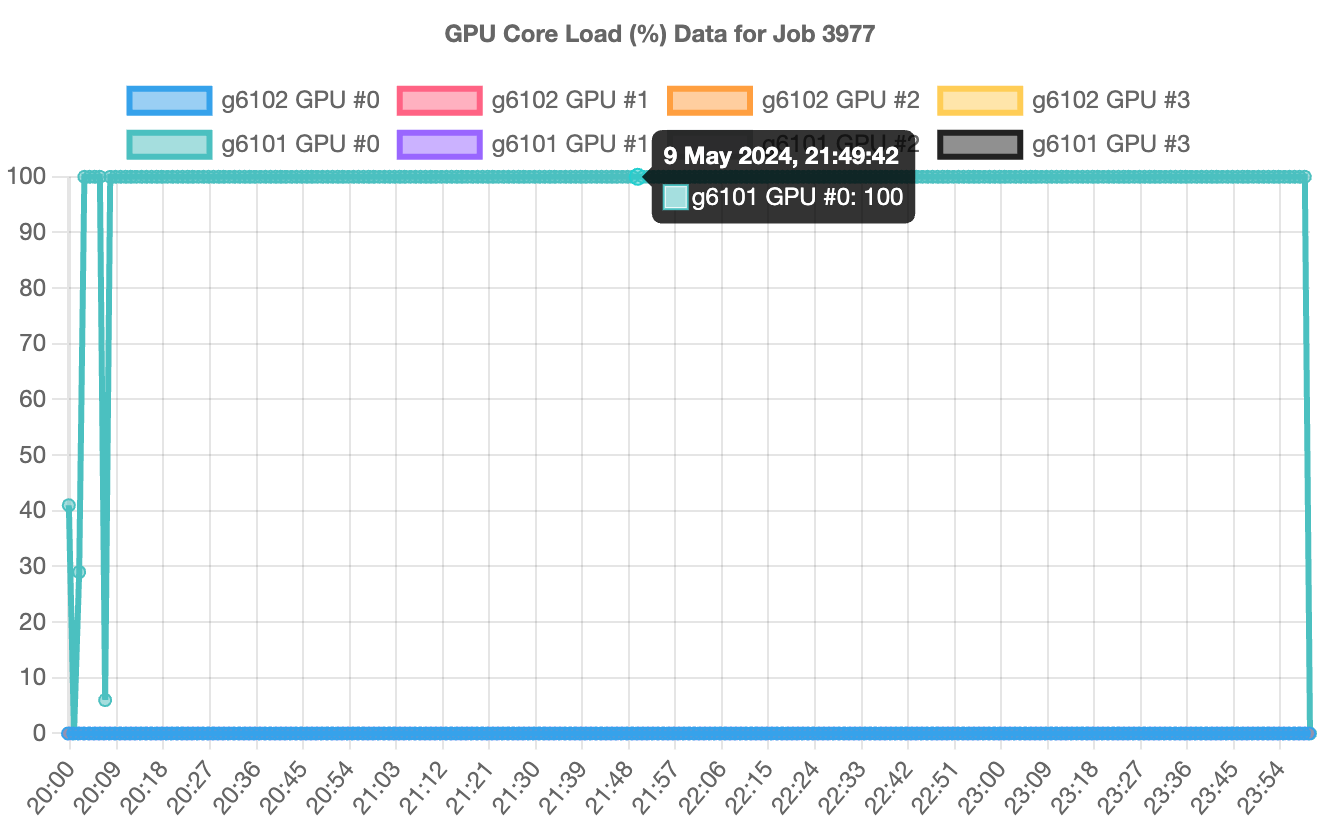
\includegraphics[width=1\textwidth]{figures/job-config-error.png}
    \caption{Job usage graph for a job with configuration error}
    \label{fig_job_config_error}
\end{figure}

\subsubsection{Code Bugs}
In another scenario, the support team received similar alerts about a job allocated multiple GPUs, described in the \textit{Configuration Error} above. Still, it showed low utilization on all GPUs except a few. Those with high usage constantly change and take turns, as Figure \ref{fig_job_code_bugs} demonstrates. By analyzing the job's execution patterns and checking with the user, they found that the workload was not adequately distributed across the GPUs because of code bugs and how the user's code was written. The user was advised to improve their code to parallelize tasks and fully utilize the allocated GPUs. This resulted in significantly improved performance and more efficient use of the cluster's GPU resources.

\begin{figure}[H]
    \centering
    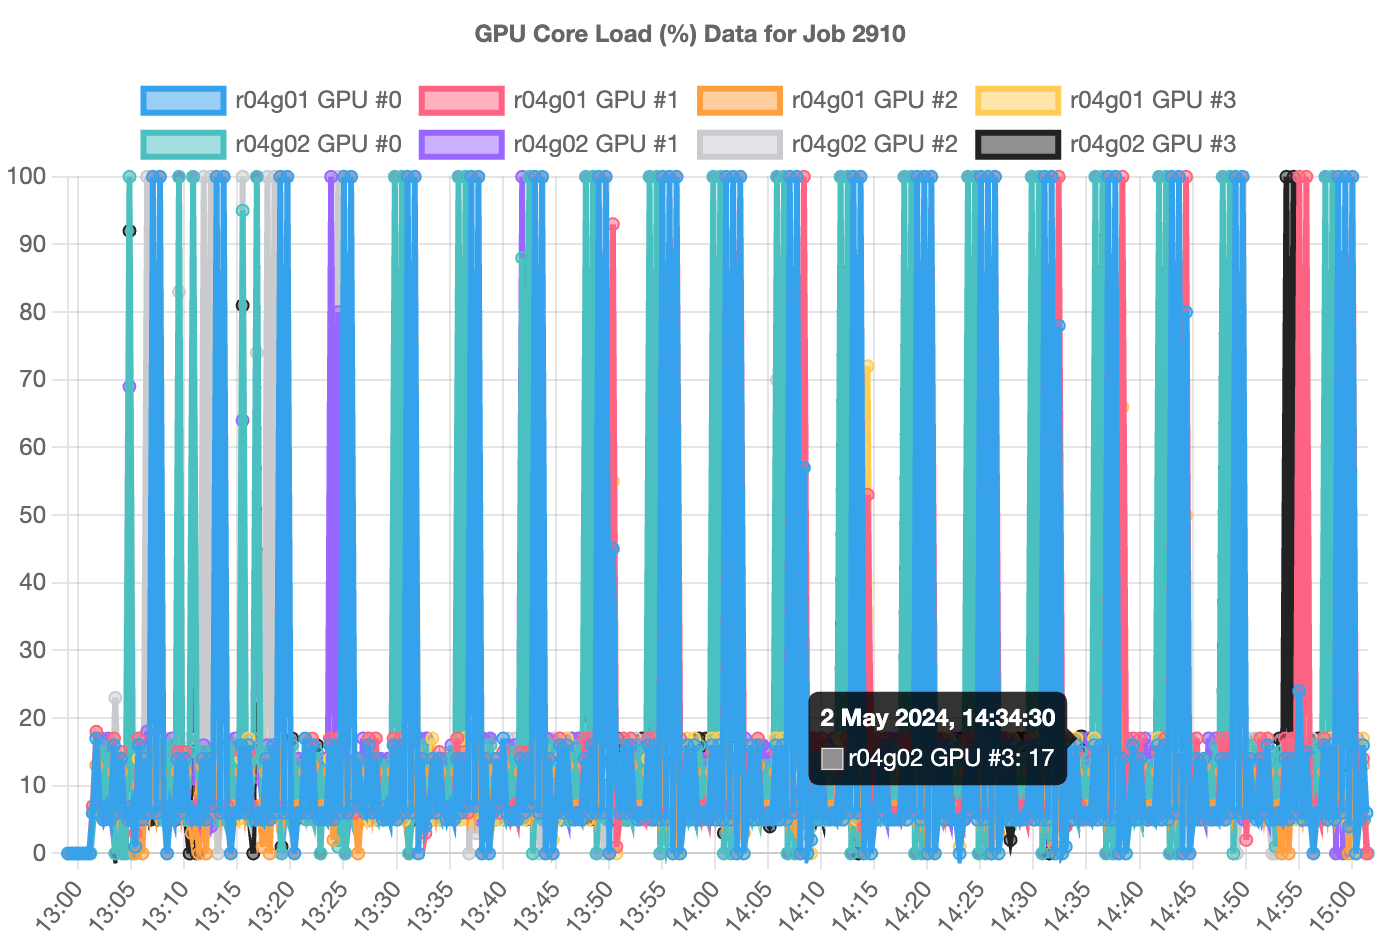
\includegraphics[width=1\textwidth]{figures/job-code-bugs.png}
    \caption{Job usage graph for a job with code bugs}
    \label{fig_job_code_bugs}
\end{figure}

\subsubsection{GPU Over-Provisioning}
For most cases, the support team was alerted by jobs with low overall GPU utilization across all allocated GPUs, as shown in Figure \ref{fig_gpu-usage-graph} and Figure \ref{fig_job_over_provison} for examples. After contacting the users, most of the time, it was found that their applications did not scale well beyond a certain number of GPUs, which means there were more allocated GPUs than needed, resulting in under-utilization of the resources. Ultimately, the support team recommended shrinking the GPU requests to match the application's needs better, leading to more efficient GPU usage and freeing for other jobs.

\begin{figure}[H]
    \centering
    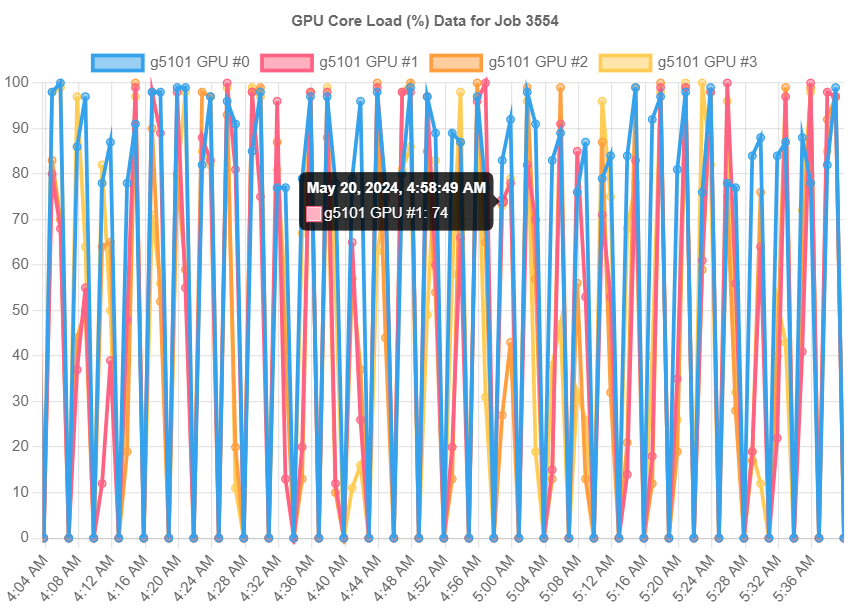
\includegraphics[width=1\textwidth]{figures/job-over-provison.png}
    \caption{Job usage graph for a job with over-provisioning}
    \label{fig_job_over_provison}
\end{figure}

\subsubsection{Interactive use on GPU compute node}
For some cases, the support team also gets alerted by jobs that only requested 1 GPU but still have low GPU utilization, on partitions meant for heavy GPU computing jobs, as demonstrated in Figure \ref{fig_job_interactive} for one example. After checking with the users, most of the time, it was found that they develop their code interactively. The user was then advised to switch their job to the partition meant for lightweight GPU computing.

\begin{figure}[H]
    \centering
    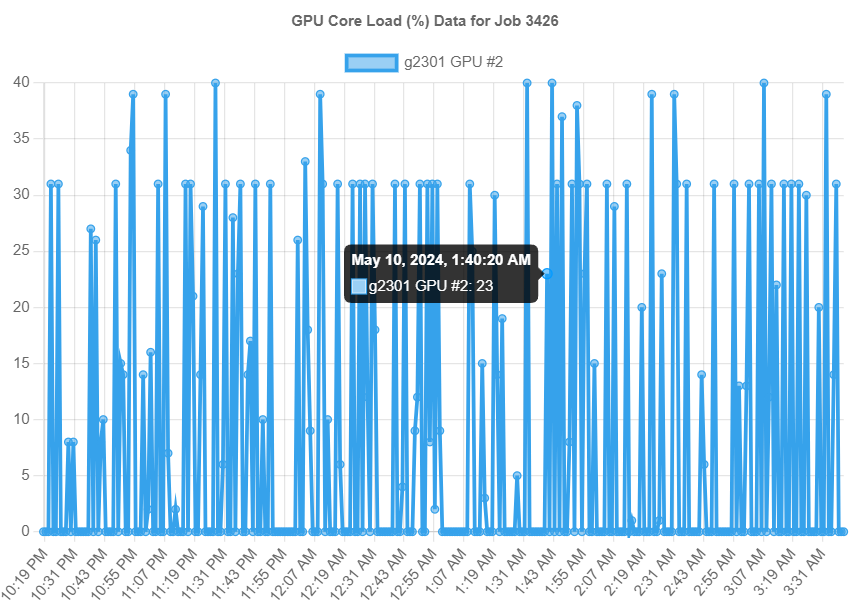
\includegraphics[width=1\textwidth]{figures/job-interactive.png}
    \caption{Job usage graph for a interactive job on heavy GPU compute partition}
    \label{fig_job_interactive}
\end{figure}

\subsubsection{GPU Memory Leaks}
A user raised a ticket, asking for help from the user support team about why his long-running AI inference job eventually crashed after some time. After checking the monitoring history, as shown in Figure \ref{fig_job_memory_leak}, the support team found progressively increasing GPU memory usage, ultimately leading to the job being killed due to exceeding memory limits. The support team worked with the user to review the code and identified a memory leak, caused by improper handling of GPU memory allocations in a loop. The memory usage was stabilized by fixing the code, allowing the job to be finished successfully, without exceeding memory limits.

\begin{figure}[H]
    \centering
    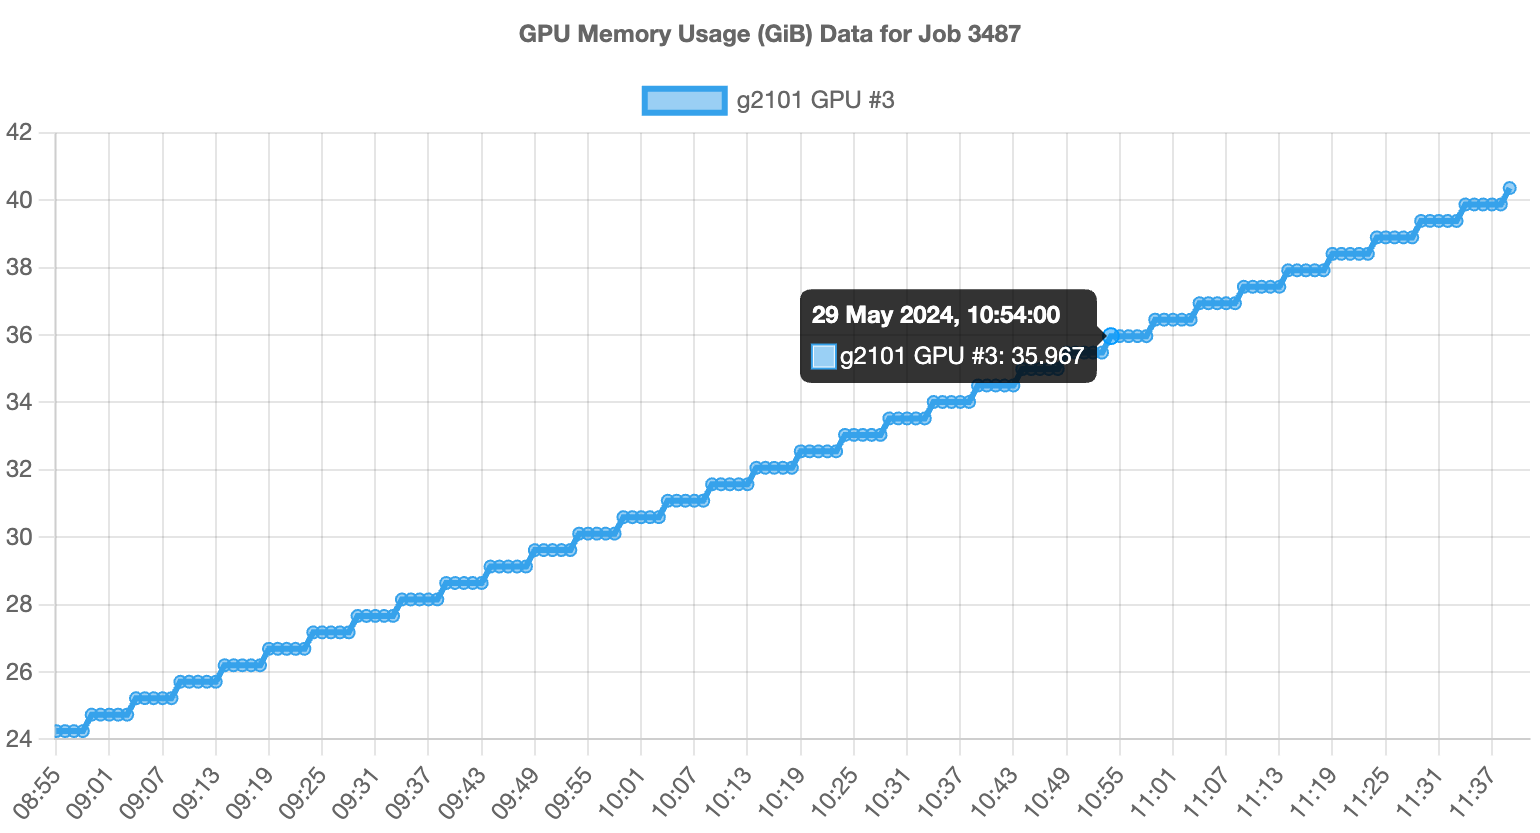
\includegraphics[width=1\textwidth]{figures/job-memory-leak.png}
    \caption{Job usage graph for a job with GPU memory leaks}
    \label{fig_job_memory_leak}
\end{figure}
